Die Datensätze $X$ (Karten) und $Y$ (Satellitenbilder) werden durch die Generatoren $G: X\rightarrow Y$ und $F: Y\rightarrow X$ sowie die Diskriminatoren $D_X$ und $D_Y$ repräsentiert, die jeweils darauf abzielen, Bilder in den Domänen $X$ und $Y$ zu unterscheiden. Die Hyperparameter wurden initial gemäß den Angaben in der Originalarbeit von Zhu et al. \cite{Zhu.2017} festgelegt und nachfolgend durch explorative Anpassungen basierend auf der Bildqualität und der Genauigkeit der Diskriminatoren verfeinert. Die Evaluierung der Leistungsfähigkeit erfolgt nach dem Training anhand einer definierten Anzahl von Testdaten.
\\\newline
Ein schwieriges Problem für die Generatoren ist die Wiedergabe feiner und detaillierter Strukturen. Insbesondere ist festzustellen, dass die Generatoren bei der Erzeugung von Straßenlinien effizienter sind. Dies ist auf die Überrepräsentation von Straßen und Häusern in den Trainingsdaten zurückzuführen. Dagegen stellt die Vielfalt der Bilder, wie Flüsse und Wälder, eine Herausforderung dar. Die genaue Erfassung der Struktur und Farbcodierung dieser Gebiete stellt die Generatoren vor Schwierigkeiten. Das Ergebnis ist oft die Generierung von Flächen mit ähnlichen Farben wie Straßen, wobei versucht wird, kleine Straßen auf der Basis dieser großen offenen Flächen zu generieren.
\\
Die Anwendung eines anderen Datensatzes, 'zebra2horse', zeigt ähnliche Herausforderungen. Die Umwandlung eines Pferdes in ein Zebra bereitet dem Generator weniger Schwierigkeiten als die umgekehrte Umwandlung. Es ist einfacher, Strukturen auf eine homogene Pferdefläche zu projizieren als unterschiedliche Kontraste und Muster auf eine homogene Zebrafläche.
\\\newline
Die Wahl der Lernrate erwies sich als kritisch, wobei die besten Ergebnisse mit einer Lernrate von $0,0002$ erzielt wurden. Diese Einstellung führte zu den höchsten SSIM-Werten und Diskriminator-Testgenauigkeiten. Insbesondere erzielte der Generator $F$ einen SSIM-Score von $0.592$, während der Generator $G$ einen Wert von $0.198$ erreichte. Die Diskriminatoren zeigten mit $50.1\%$ für $D_Y$ und $48.5\%$ für $D_X$ nahezu optimale Genauigkeiten. Trotz der auf den ersten Blick großen visuellen Ähnlichkeit der generierten Satellitenbilder zeigte eine genauere Analyse, dass kleinere Strukturen im generierten Bild fehlten. Dies spiegelte sich im vergleichsweise niedrigen SSIM-Wert wider.
\\\newline
Bei einem Gewichtungsfaktor von $\lambda = 120$ wurden sowohl bei der visuellen Beurteilung als auch beim SSIM-Score die besten Ergebnisse erzielt.
Die Abbildung \ref{evaluation:cycleGan_Testergebnisse} zeigt einen Teil der Ergebnisse.
Dieser spezifische Wert für $\lambda$ führte zu erzeugten Bildern, deren Signal-Rausch-Verhältnis (SNR) entweder besser oder nahezu gleich dem des Originalbildes war. Der SNR-Wert gibt das Verhältnis zwischen dem Signal, repräsentiert durch relevante Bildinformationen, und dem Rauschen, repräsentiert durch unerwünschte Störungen, an. Ein höherer SNR-Wert bedeutet eine bessere Bildqualität und Klarheit gegenüber dem Rauschen.

\begin{figure}[ht]
  \begin{subfigure}[t]{.14\textwidth}
    \centering
    \caption*{Input}
    
\includegraphics[width=\linewidth]{images/cycleGanResults/Maps19_Or_Ld120_E100_Lr0002.jpg}
  \end{subfigure}
  \begin{subfigure}[t]{.14\textwidth}
    \centering
    \caption*{Output}
    
\includegraphics[width=\linewidth]{images/cycleGanResults/Maps19Ld120_E100_Lr0002.jpg}
  \end{subfigure}
  \begin{subfigure}[t]{.14\textwidth}
    \centering
    \caption*{Differenzbild}
    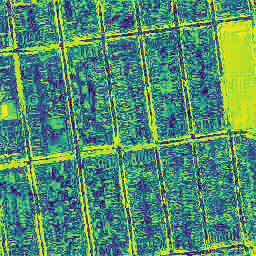
\includegraphics[width=\linewidth]{images/cycleGanResults/Maps9_diff.png}
  \end{subfigure}
  \hfill
  \begin{subfigure}[t]{.14\textwidth}
    \centering
    \caption*{Input}
    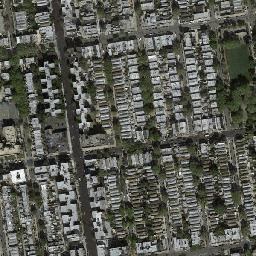
\includegraphics[width=\linewidth]{images/cycleGanResults/Satelite19_Or_Ld120_E100_Lr0002.jpg}
  \end{subfigure}
  \begin{subfigure}[t]{.14\textwidth}
    \centering
    \caption*{Output}
    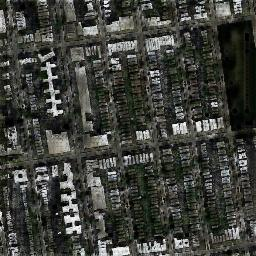
\includegraphics[width=\linewidth]{images/cycleGanResults/Satelite19Ld120_E100_Lr0002.jpg}
  \end{subfigure}
  \begin{subfigure}[t]{.14\textwidth}
    \centering
    \caption*{Differenzbild}
    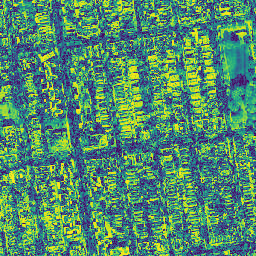
\includegraphics[width=\linewidth]{images/cycleGanResults/Satelite2_diff.png}
  \end{subfigure}

  \medskip

  \begin{subfigure}[t]{.14\textwidth}
    \centering
    
\includegraphics[width=\linewidth]{images/cycleGanResults/Maps8_Or_Ld120_E100_Lr0002.jpg}
  \end{subfigure}
  \begin{subfigure}[t]{.14\textwidth}
    \centering
    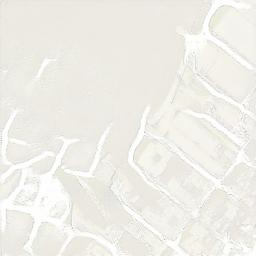
\includegraphics[width=\linewidth]{images/cycleGanResults/Maps8_Ld120_E100_E0002.jpg}
  \end{subfigure}
  \begin{subfigure}[t]{.14\textwidth}
    \centering
    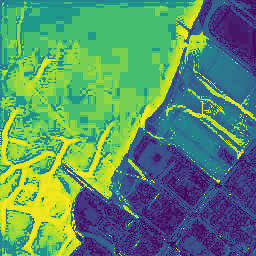
\includegraphics[width=\linewidth]{images/cycleGanResults/Maps6_diff.png}
  \end{subfigure}
  \hfill
  \begin{subfigure}[t]{.14\textwidth}
    \centering
    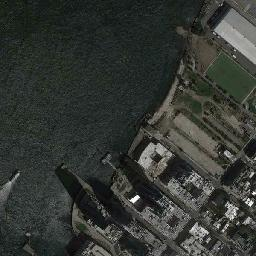
\includegraphics[width=\linewidth]{images/cycleGanResults/Satelite8_Or_Ld120_E100_Lr0002.jpg}
  \end{subfigure}
  \begin{subfigure}[t]{.14\textwidth}
    \centering
    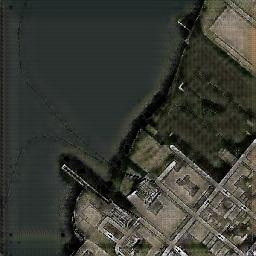
\includegraphics[width=\linewidth]{images/cycleGanResults/Satelite8_Ld120_E100_E0002.jpg}
  \end{subfigure}
  \begin{subfigure}[t]{.14\textwidth}
    \centering
    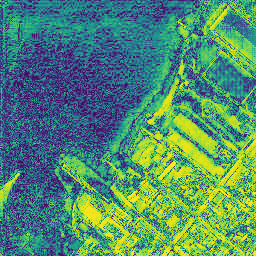
\includegraphics[width=\linewidth]{images/cycleGanResults/Satelite1_diff.png}
  \end{subfigure}
  \caption{Testergebnisse nach dem Training mit $\lambda=120$, Lernrate $=0.0002$ und $100$ Epochen}
  \label{evaluation:cycleGan_Testergebnisse}
\end{figure}

\begin{figure}[H]
  \begin{subfigure}[t]{.45\textwidth}
    \centering
    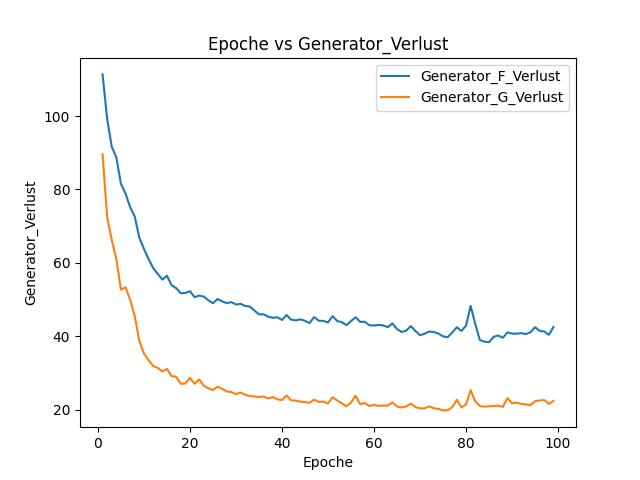
\includegraphics[width=\linewidth]{images/cycleGanResults/Generator_Verlust.jpg}
  \end{subfigure}
  \hfill
  \begin{subfigure}[t]{.45\textwidth}
    \centering
    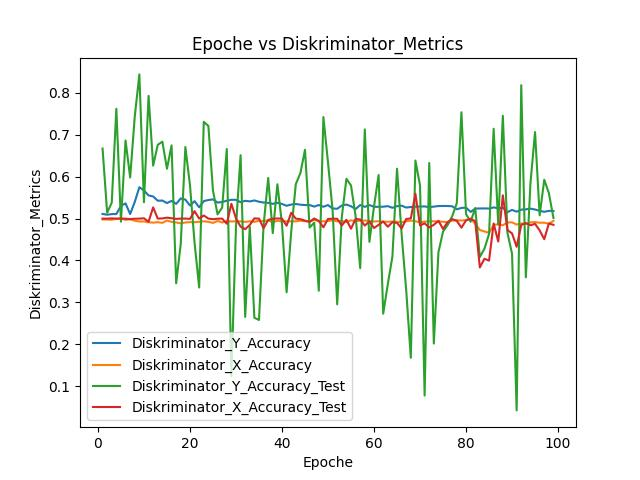
\includegraphics[width=\linewidth]{images/cycleGanResults/Diskriminator_Metrics.jpg}
  \end{subfigure}
  \medskip
  \begin{subfigure}[t]{.45\textwidth}
    \centering
    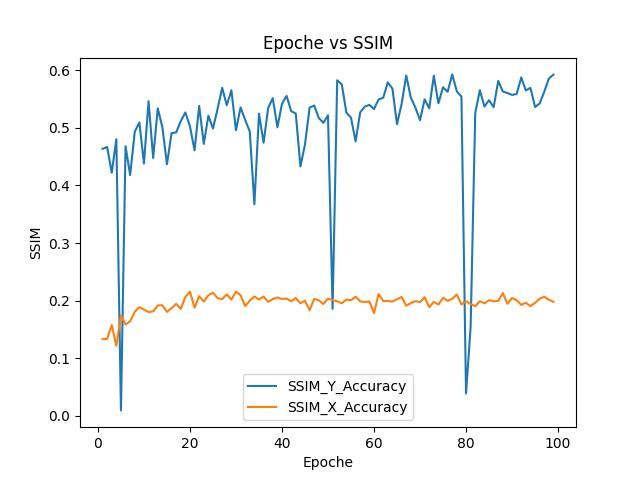
\includegraphics[width=\linewidth]{images/cycleGanResults/SSIM.jpg}
  \end{subfigure}
  \hfill
  \begin{subfigure}[t]{.45\textwidth}
    \centering
    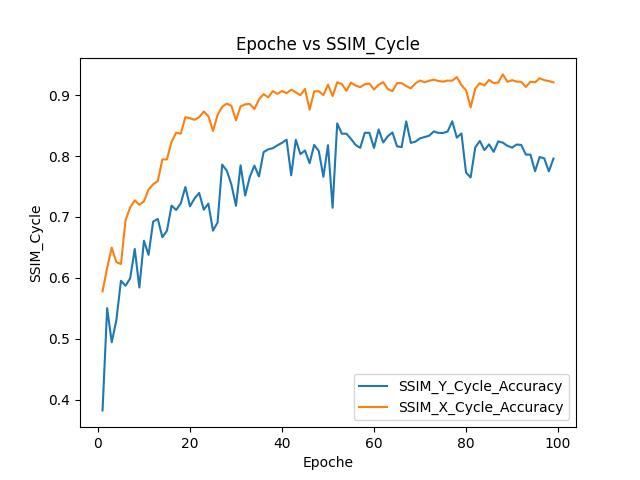
\includegraphics[width=\linewidth]{images/cycleGanResults/SSIM_Cycle.jpg}
  \end{subfigure}

  \caption{Verlauf der Metriken beim Training mit $\lambda=120$, Lernrate $=0.0002$ und $100$ Epochen. Die Metriken umfassen: Generator-Verlust (oben links), Diskriminator-Genauigkeiten auf den Trainings- und Testdaten (oben rechts), sowie SSIM-Score (unten links) und Zyklus-SSIM-Score (unten rechts).
  Die Metriken werden in Abhängigkeit von der Anzahl der Epochen auf der x-Achse untersucht.}
  \label{evaluation:cycleGan_Metriken}
\end{figure}

Trotz dieser Erfolge bleibt das Training instabil, und es besteht die Möglichkeit eines Modekollapses. Die Generatoren zeigen Anzeichen eines exponentiellen Verfalls in ihren Verlustkurven, während der SSIM-Score nur langsam ansteigt (Abbildung \ref{evaluation:cycleGan_Metriken}). Dies deutet darauf hin, dass die Generatoren zwar ihre Verluste minimieren, jedoch möglicherweise nicht die gewünschte visuelle Qualität erreichen.\\

\begin{figure}
  \begin{subfigure}[t]{.2\textwidth}
    \caption{Input}
    \centering
    
\includegraphics[width=\linewidth]{images/cycleGanResults/Maps10_Or_Ld120_E100_Lr0002.jpg}
  \end{subfigure}
  \begin{subfigure}[t]{.2\textwidth}
    \caption{Output}
    \centering
    
\includegraphics[width=\linewidth]{images/cycleGanResults/Maps10_Ld120_E100_Lr0002.jpg}
  \end{subfigure}
  \hfill
  \begin{subfigure}[t]{.2\textwidth}
    \caption{Input}
    \centering
    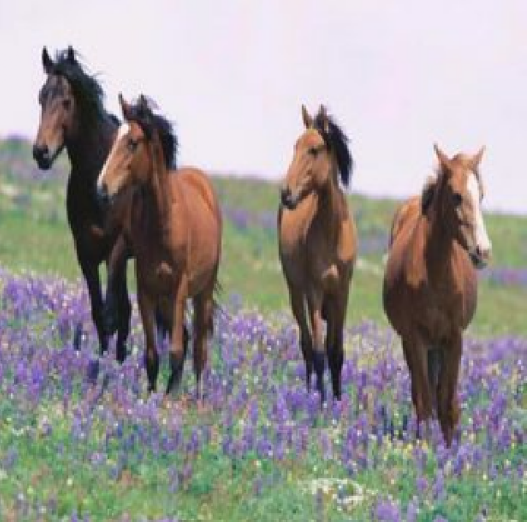
\includegraphics[width=\linewidth]{images/cycleGanResults/horse_input1.png}
  \end{subfigure}
  \begin{subfigure}[t]{.2\textwidth}
    \caption{Output}
    \centering
    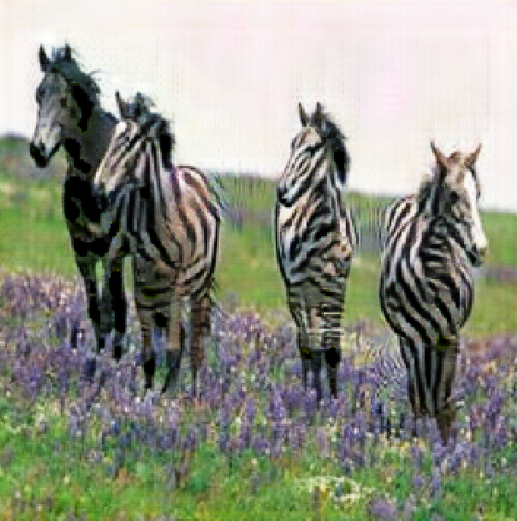
\includegraphics[width=\linewidth]{images/cycleGanResults/horse_output1.png}
  \end{subfigure}

  \medskip

  \begin{subfigure}[t]{.2\textwidth}
    \centering
    
\includegraphics[width=\linewidth]{images/cycleGanResults/Maps6_Or_Ld120_E100_Lr0002.jpg}
  \end{subfigure}
  \begin{subfigure}[t]{.2\textwidth}
    \centering
    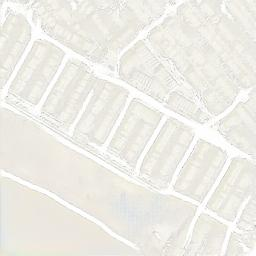
\includegraphics[width=\linewidth]{images/cycleGanResults/Maps6Ld120_E100_Lr0002.jpg}
  \end{subfigure}
  \hfill
  \begin{subfigure}[t]{.2\textwidth}
    \centering
    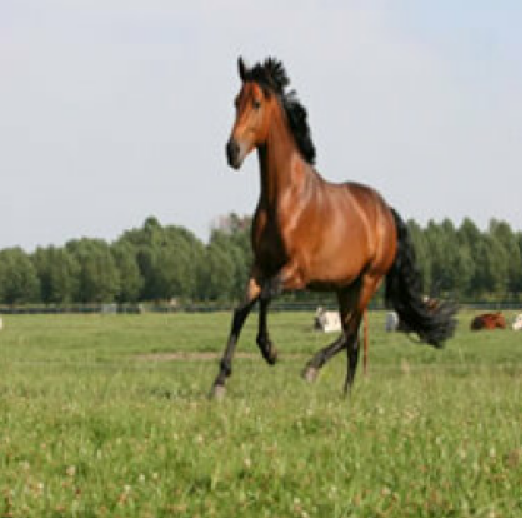
\includegraphics[width=\linewidth]{images/cycleGanResults/horse_input2.png}
  \end{subfigure}
  \begin{subfigure}[t]{.2\textwidth}
    \centering
    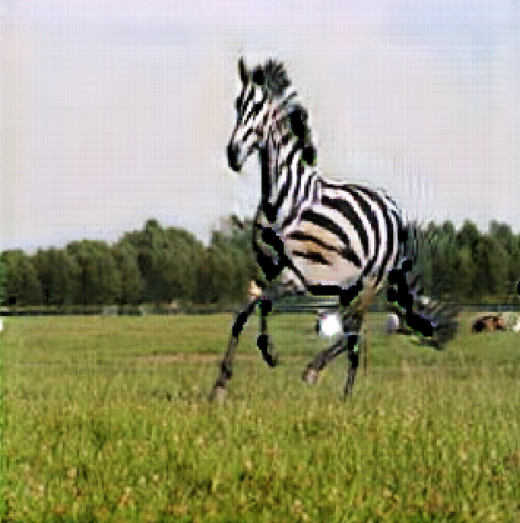
\includegraphics[width=\linewidth]{images/cycleGanResults/horse_output2.png}
  \end{subfigure}

  \medskip

  \begin{subfigure}[t]{.2\textwidth}
    \centering
    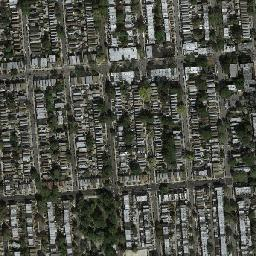
\includegraphics[width=\linewidth]{images/cycleGanResults/Satelite10_Or_Ld120_E100_Lr0002.jpg}
  \end{subfigure}
  \begin{subfigure}[t]{.2\textwidth}
    \centering
    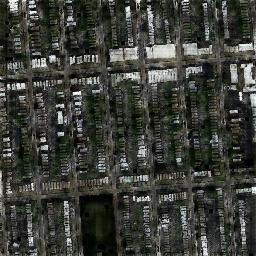
\includegraphics[width=\linewidth]{images/cycleGanResults/Satelite10_Ld120_E100_Lr0002.jpg}
  \end{subfigure}
  \hfill
  \begin{subfigure}[t]{.2\textwidth}
    \centering
    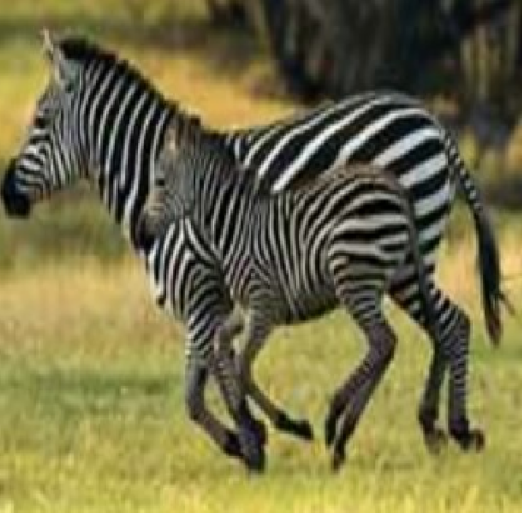
\includegraphics[width=\linewidth]{images/cycleGanResults/zebra_input1.png}
  \end{subfigure}
  \begin{subfigure}[t]{.2\textwidth}
    \centering
    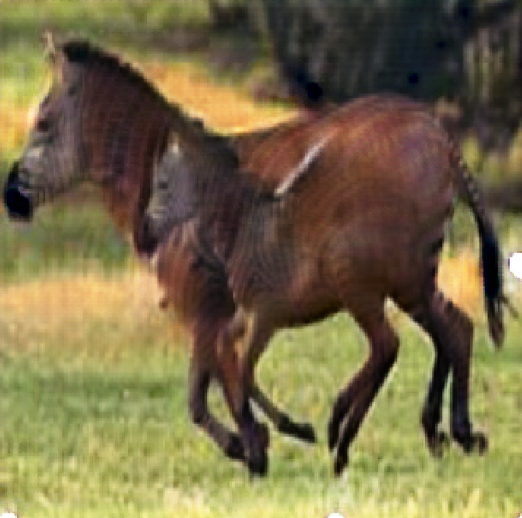
\includegraphics[width=\linewidth]{images/cycleGanResults/zebra_output1.png}
  \end{subfigure}

  \medskip

  \begin{subfigure}[t]{.2\textwidth}
    \centering
    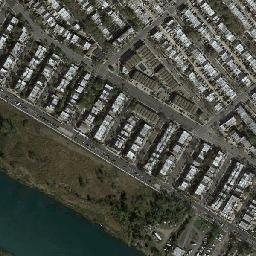
\includegraphics[width=\linewidth]{images/cycleGanResults/Satelite6_Or_Ld120_E100_Lr0002.jpg}
  \end{subfigure}
  \begin{subfigure}[t]{.2\textwidth}
    \centering
    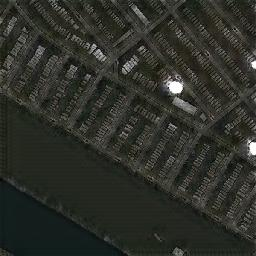
\includegraphics[width=\linewidth]{images/cycleGanResults/Satelite6Ld120_E100_Lr0002.jpg}
  \end{subfigure}
  \hfill
  \begin{subfigure}[t]{.2\textwidth}
    \centering
    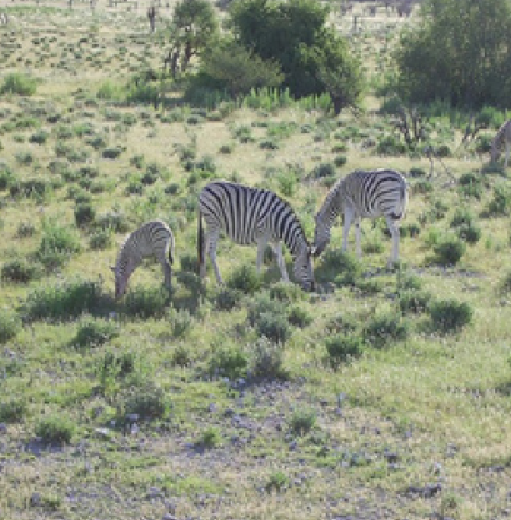
\includegraphics[width=\linewidth]{images/cycleGanResults/zebra_input2.png}
  \end{subfigure}
  \begin{subfigure}[t]{.2\textwidth}
    \centering
    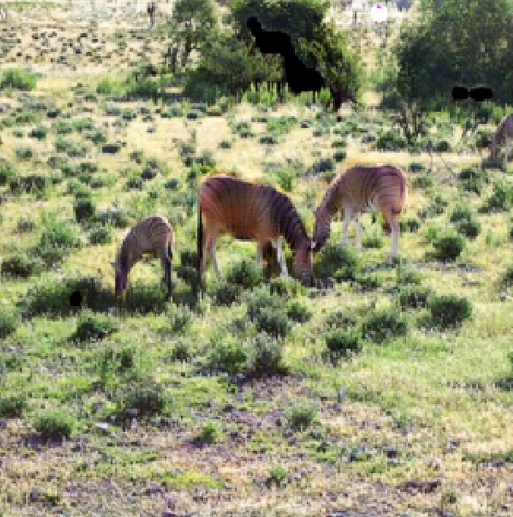
\includegraphics[width=\linewidth]{images/cycleGanResults/zebra_output2.png}
  \end{subfigure}
  \caption{CycleGAN-Ergebnisse aus verschiedenen Datensätzen}

\end{figure}


Die generierten Bilder zeigen bereits zu diesem Zeitpunkt eine grobe visuelle Ähnlichkeit mit der zugrunde liegenden Originalbildstruktur mit minimalen Abweichungen. Im SSIM-Score werden jedoch die Schwierigkeiten der Generatoren bei der Erzielung signifikanter Verbesserungen in Bezug auf feinere Details und Farbübereinstimmungen deutlich. Dies ist auch visuell an den Differenzbildern zu erkennen, die mit Hilfe eines Histogrammabgleichs kontrastverbessert wurden. Helle Bereiche in diesen Differenzbildern zeigen größere Unterschiede. Insbesondere bei kleinen pixelweisen Details sowie bei unterschiedlichen Farbkodierungen häufen sich die hellen Bereiche. Die Abbildung \ref{evaluation:cycleGan_Testergebnisse} zeigt ein solches Beispiel.
\\
Insbesondere in den frühen Epochen sind die Generatoren nicht in der Lage, Straßenlinien zuverlässig als gerade Linien zu generieren. Diese Schwächen verbessern sich mit zunehmender Trainingsdauer, so dass nach ca. 300 Epochen relativ konsistente Geraden erzeugt werden.
\\\newline
Die Analyse des SSIM-Wertes in Abhängigkeit von der Zyklusübersetzung zeigt einen exponentiellen Anstieg. Diese Beobachtung deutet darauf hin, dass der Verlust der Zykluskonsistenz einen signifikanten Einfluss auf das Training hat. Der exponentielle Anstieg des SSIM-Wertes deutet darauf hin, dass die Konsistenz zwischen den Originalbildern und den rückübersetzten Bildern mit der Zeit kontinuierlich zunimmt. Dies kann auf eine kontinuierliche Verbesserung der Generatoren hinsichtlich ihrer Fähigkeit zur Zyklusübersetzung hindeuten. Insgesamt erreichen die SSIM-Scores für die Zyklusübersetzung Werte von $80\%$ für $Y$ und $90\%$ für $X$ (Abbildung \ref{evaluation:cycleGan_Metriken}).\\

\begin{table}
\centering
\begin{tabular}{|l|l|l|l|l|l|l|l|l|l|l|l|l|l|l|}
\hline
\textbf{Lambda} &
  \textbf{Epoche} &
  \textbf{Lernrate} &
  \textbf{\begin{tabular}[c]{@{}l@{}}$D_Y$ \\ Tr-Acc\end{tabular}} &
  \textbf{\begin{tabular}[c]{@{}l@{}}$D_X$ \\ Tr-Acc\end{tabular}} &
  \textbf{\begin{tabular}[c]{@{}l@{}}$D_Y$ \\ Te-Acc\end{tabular}} &
  \textbf{\begin{tabular}[c]{@{}l@{}}$D_X$ \\ Te-Acc\end{tabular}} \\ \hline
120 & 100 & 0.000025 & 0.549 & 0.494 & 0.307 & 0.497   \\ \hline
120 & 100 & 0.00005  & 0.537 & 0.491 & 0.321 & 0.489 \\ \hline
120 & 100 & 0.0001   & 0.519 & 0.490 & 0.418 & 0.485 \\ \hline
120 & 100 & 0.0002   & 0.518 & 0.495 & 0.501 & 0.485 \\ \hline
120 & 100 & 0.0004   & 0.524 & 0.487 & 0.771 & 0.433 \\ \hline
100 & 100 & 0.0002   & 0.521 & 0.491 & 0.527 & 0.481   \\ \hline
140 & 100 & 0.0002   & 0.562 & 0.492 & 0.544 & 0.469 \\ \hline
120 & 200 & 0.0002   & 0.514 & 0.500 & 0.563 & 0.489 \\ \hline
100 & 300 & 0.0002   & 0.510 & 0.484 & 0.470 & 0.676 \\ \hline
120 & 300 & 0.0002   & 0.508 & 0.495 & 0.468 & 0.709  \\ \hline
\end{tabular}
\caption{CycleGAN Ergebnisse unter verschiedenen Hyperparametern mit Batchgröße 1, Teil1}
\label{evaluation:cycleGan_table1}
\end{table}

\begin{table}
\centering
\begin{tabular}{|l|l|l|l|l|l|l|l|l|l|l|l|l|l|l|}
\hline
\textbf{\begin{tabular}[c]{@{}l@{}}$F$\\ Loss\end{tabular}} &
\textbf{\begin{tabular}[c]{@{}l@{}}$G$\\ Loss\end{tabular}} &
  \textbf{\begin{tabular}[c]{@{}l@{}}$X$ \\ SSIM\end{tabular}} &
  \textbf{\begin{tabular}[c]{@{}l@{}}$Y$ \\SSIM \end{tabular}} &
  \textbf{\begin{tabular}[c]{@{}l@{}}$X$\\Z-SSIM\end{tabular}} &
  \textbf{\begin{tabular}[c]{@{}l@{}}$Y$ \\ Z-SSIM\end{tabular}} &
  \textbf{\begin{tabular}[c]{@{}l@{}}$X$\\SNR \end{tabular}} &
  \textbf{\begin{tabular}[c]{@{}l@{}}$Y$\\SNR\end{tabular}} \\ \hline
53.113 & 22.556 & 0.545 & 0.191 & 0.895 & 0.831 & -2.991 & 0.228  \\ \hline
44.626 & 20.417 & 0.541 & 0.191 & 0.916 & 0.836 & -0.589 & 1.071  \\ \hline
44.376 & 21.943 & 0.580 & 0.194 & 0.935 & 0.842 & -4.604 & 1.367  \\ \hline
42.489 & 22.373 & 0.592 & 0.198 & 0.921 & 0.796 & -5.308 & 0.851  \\ \hline
47.239 & 29.084 & 0.588 & 0.207 & 0.601 & 0.845 & -2.407 & 0.823\\ \hline
34.973 & 18.837 & 0.551 & 0.194 & 0.930 & 0.830 & -3.292 & 1.261  \\ \hline
13.048 & 6.842  & 0.510 & 0.179 & 0.513 & 0.409 & -2.087 & 1.005  \\ \hline
46.061 & 23.058 & 0.371 & 0.177 & 0.802 & 0.894 & 1.915	 & 1.992 \\\hline
34.881 & 20.899 & 0.577 & 0.191 & 0.931 & 0.756 & -2.705 & 1.373  \\ \hline
46.652 & 26.360 & 0.585 & 0.207 & 0.901 & 0.707 & -3.409 & 1.248\\ \hline
\end{tabular}
\caption{CycleGAN Ergebnisse unter verschiedenen Hyperparametern mit Batchgröße 1, Teil2}
\label{evaluation:cycleGan_table2}
\end{table}


Im Gegensatz dazu bleibt die Genauigkeit der Diskriminatoren für die Trainingsdaten stabil bei etwa $50\%$. Für die Testdaten, insbesondere für $D_Y$, sind jedoch erhebliche Schwankungen in Abhängigkeit von der Epoche festzustellen  (Abbildung \ref{evaluation:cycleGan_Metriken}). Dies deutet darauf hin, dass die Diskriminatoren möglicherweise Schwierigkeiten haben, mit neuen, untrainierten Daten umzugehen. Diese Schwankungen können auf eine Überanpassung oder eine mangelnde Generalisierungsfähigkeit des Modells hinweisen, trotz der implementierten Maßnahmen wie dem Hinzufügen von Rauschen und Dropout-Schichten.\\\newline
Die Trainingszeit spiegelt die Komplexität der Modelle wider, insbesondere auf der GPU, wo jede Epoche im Durchschnitt etwa 2 Minuten dauert. Im Vergleich dazu benötigt die CPU, selbst nach Reduktion der Residualblöcke auf einen Block, etwa 6 Minuten pro Epoche. Die Verwendung der Instanznormalisierung trägt zur Beschleunigung der Konvergenz und zur Verbesserung der Laufzeit bei. Auch im Vergleich zu Generatoren mit zusätzlichen Schichten zeigt sich, dass die Verwendung von Restblöcken eine bessere Laufzeit ermöglicht. 
\\\newline
Insgesamt zeigt die Evaluierung, dass das CycleGAN-Modell trotz einiger Herausforderungen bei der Generierung detaillierter Strukturen und der Generalisierung auf neue Daten vielversprechende Ergebnisse liefert.